% Das Buch ist lizensiert unter der Creative-Commons-Lizenz
% "Namensnennung 4.0 International (CC BY 4.0)"
% http://creativecommons.org/licenses/by/4.0/deed.de

\chapter{Zusammengesetzte Daten}
\label{cha:zusammengesetzte-daten}

Viele Informationen, die in Programmen repräsentiert werden, bestehen
aus mehreren Bestandteilen:
%
\begin{itemize}
\item Ein Festessen besteht aus Vorspeise, Hauptgang und Nachspeise.
\item Eine Uhrzeit besteht aus Stunde und Minute.
\item Eine Tür besteht aus Türblatt und Türgriff.
\end{itemize}
%
Es werden also mehrere Dinge zu einem \textit{zusammengesetzt}.
Eine andere Betrachtungsweise ist, dass ein einzelnes
Ding \textit{mehrere Eigenschaften} hat:
%
\begin{itemize}
\item Ein Filzstift hat Dicke und Farbe.
\item Eine Katze hat Alter und Geschlecht.
\item Ein Lautsprecher hat Minimal- und Maximalfrequenz.
\end{itemize}
%
Um solche Informationen abzubilden, führt dieses Kapitel eine neue Art
Daten ein, die \textit{zusammengesetzten
  Daten}\index{zusammengesetzten Daten}.

\section{Computer konfigurieren}
\label{sec:computer-konfigurieren}

Viele Computerhändler erlauben ihren Kunden, bestimmte Komponenten
eines neues Computers selbst auszuwählen, zum Beispiel den Prozessor,
die Festplatte oder die Größe des RAM"=Hauptspeichers:
%
\begin{center}
  \medskip
  \includegraphics[height=0.3\textheight]{computer}
  \medskip
\end{center}
%
Anders gesagt, der Computer ein Computer\index{Computer} \emph{besteht aus}:
%
\begin{itemize}
\item Prozessor
\item RAM
\item Festplatte
\end{itemize}
%
Natürlich besteht ein Computer auch noch aus anderen Teilen, die
aber (zumindest in diesem Beispiel) immer gleich sind.  In einer Bestellung muß
die Kundin also nur diese drei Bestandteile angeben.  Wir nehmen an,
dass es beim Prozessor nur auf den Namen ("`Athlon"', "`Xeon"',
"`Cell"', \ldots) ankommt, beim RAM nur auf die Größe in Gigabyte, und
auch bei der Festplatte nur auf die Größe in Gigabyte.  Eine
vereinfachte Darstellung könnte so aussehen:
%
\begin{center}
  Computer:
  \begin{tabular}[c]{r|l}
    \textbf{Feld} & \textbf{Komponente}\\\hline
    \hline
     Prozessor & \verb|"Cell"|\\
     \hline
     RAM & 8\\
    \hline 
    Festplatte & 250
  \end{tabular}
\end{center}
%
Diese Tabelle steht demnach für einen Computer mit Cell-Prozessor, 8
Gigabyte RAM und einer 250-Gigabyte-Festplatte~-- sie hat mehrere
Bestandteile und ist damit zusammengesetzt.  Der Computerhändler wird
viele Computer nach diesem Schema ausliefern, bei denen allesamt
Prozessor, RAM und Festplatte von den Kundinnen bestimmt wird.  Solche
Informationen, die alle dem gleichen Schema folgen, können also nach
"`Typ"' sortiert werden, wobei der Typ
festlegt, um was für eine Art Information es geht und aus welchen
Teilen sie zusammengesetzt ist.  In der obigen Tabelle ist das
\textit{Feld} die Allgemeinbezeichnung für ein Bestandteil, das
alle Computer haben.  Die \textit{Komponente} ist das konkrete
Bestandteil eines einzelnen Computers.

Zusammengesetzte Daten bilden die DeinProgramm-Sprachen durch
sogenannte \textit{Records}\index{Records} ab.  Jeder Record gehört
zu einem bestimmten
\textit{Record-Typ\index{Record-Typ}}, der festlegt, was für eine
Sorte Information repräsentiert wird und welche Felder des Records
des Typs haben.

\begin{verbatim}
(define-record-functions computer
  make-computer
  (computer-processor  string)
  (computer-ram        rational)
  (computer-hard-drive rational))
\end{verbatim}

Der Record-Typ für Computer sieht feste Felder\index{Feld}
vor ("`Prozessor"', "`RAM"' und "`Festplatte"').  Ein einzelner Record
dieses Typs besteht aus Komponenten\index{Komponente}, eine pro
Feld. (In diesem Fall "`\texttt{Cell}"', $8$ und $250$.)
Der Record-Typ für Computer ist in der DeinProgramm-Sprachen
\texttt{Anfänger} eingebaut.\footnote{Weiter hinten in diesem Kapitel
  beschreiben wir, wie ein Programm eigene Record-Typen definieren
  kann.}

Für jeden Record-Typ gibt es Funktionen, mit denen Records
zusammengebaut und auch wieder auseinandergenommen werden können.
Analog zum Zusammenbauen eines Computer mit Cell-Prozessor, 8 Gigabyte
RAM und 250 Gigabyte Festplatte wird der dazugehörige Record mit der
eingebauten Funktion \texttt{make-computer} folgendermaßen
hergestellt:
%
\begin{alltt}
(make-computer "Cell" 8 250)
\evalsto{} #<record:computer "Cell" 8 250>
\end{alltt}
%
\texttt{Make-computer} hat folgende Signatur:
%
\begin{alltt}
(: make-computer (string rational rational -> computer))
\end{alltt}
%
Die drei Eingaben sind respektive Prozessor, RAM und Festplatte.
\texttt{Make-computer} macht daraus einen Wert der eingebauten Sorte
\texttt{computer} der Computer-Records.  Da \texttt{make-computer}
einen Computer-Record "`konstruiert"', heißt die Funktion auch
\textit{Konstruktor\index{Konstruktor}}.

Mit der Schreibweise
%
\begin{verbatim}
#<record:... ...>
\end{verbatim}
%
werden Record-Typ und Komponenten sichtbar.

Computer-Records sind Werte wie andere auch und lassen sich zum Beispiel an
Variablen binden:
%
\begin{alltt}
; Cell, 4 Gbyte RAM, 1000 Gbyte Festplatte
(define gamer (make-computer "Cell" 4 1000))

gamer
\evalsto{} #<record:computer "Cell" 4 1000>
; Xeon, 2 Gbyte RAM, 500 Gbyte Festplatte
(define workstation (make-computer "Xeon" 2 500))

workstation
\evalsto{} #<record:computer "Xeon" 2 500>
\end{alltt}
%
Umgekehrt zur Konstruktion nehmen manche Bastler aus dem Computer die
Einzelteile wieder heraus, zum Beispiel, um sie in einem anderen
Computer zu verbauen. Für dieses Herausnehmen sind die Funktionen
\texttt{computer"=processor}, \texttt{computer"=ram} und
\texttt{computer-hard-drive} zuständig:
%
\begin{alltt}
(computer-processor gamer)
\evalsto{} "Cell"
(computer-ram gamer)
\evalsto{} 4
(computer-hard-drive gamer)
\evalsto{} 1000
\end{alltt}
%
Diese drei Funktionen heißen \textit{Selektoren\index{Selektor}}.  Sie haben
folgende Signaturen:
%
\begin{alltt}
(: computer-processor (computer -> string))
(: computer-ram (computer -> rational))
(: computer-hard-drive (computer -> rational))
\end{alltt}
%
Mit Hilfe des Konstruktors und der Selektoren kann der Programmierer
weitergehende Funktionen definieren.  Für den Anfang könnte das
eine Funktion sein, die den Gesamtspeicher eines Computers berechnet,
also Hauptspeicher und Festplattenspeicher zusammen.
Eine solche Funktion müßte Kurzbeschreibung und Signatur wie folgt haben:\index{total-memory@\texttt{total-memory}}
%
\begin{alltt}
; Gesamtspeicher berechnen
(: total-memory (computer -> rational))
\end{alltt}
%
Hier sind unsere Erwartungen an \texttt{total-memory}, als Testfälle
formuliert:
%
\begin{alltt}
(check-expect (total-memory workstation) 502)
(check-expect (total-memory gamer) 1004)
\end{alltt}
% 
Das Gerüst müßte folgendermaßen sein:
%
\begin{alltt}
(define total-memory
  (lambda (c)
    ...))
\end{alltt}
%
Um etwas aus dem Record zu berechnen, muss \texttt{total-memory} (und
so gut wie jede andere Funktion auch) die Bestandteile betrachten.  Es
ist deshalb sinnvoll, die Schablone mit den Aufrufe der Selektoren zu
bestücken.
%
\begin{alltt}
(define total-memory
  (lambda (c)
    ... (computer-processor c) ...
    ... (computer-ram c) ...
    ... (computer-hard-drive c) ...))
\end{alltt}
%
Jetzt wo die Schablone fertig ist, können wir uns mit dem Inhalt der
Aufgabe beschäftigen: Der Prozessor hat nichts mit der
Speichermenge zu tun, wir können den entsprechenden Selektoraufruf
also wieder löschen:
%
\begin{alltt}
(define total-memory
  (lambda (c)
    ... (computer-ram c) ...
    ... (computer-hard-drive c) ...))
\end{alltt}
%
Das Gesamtspeicher ergibt sich aus Addition der beiden Komponenten:
%
\begin{alltt}
(define total-memory
  (lambda (c)
    (+ (computer-ram c)
       (computer-hard-drive c))))
\end{alltt}
%
Fertig!

\texttt{Total-memory} ist ein Beispiel für eine Funktion, die einen
Record akzeptiert.  Umgekehrt gibt es auch Funktionen, die Records
produzieren.  Angenommen, unser Computerhändler bietet neben der
Einzelkonfiguration von Prozessor, Hauptspeicher und Festplatte einige
Standardmodelle an~-- sagen wir, ein Billigmodell, ein Modell für
Profis (was immer eine "`Profi"' sein mag) und ein Modell für
Computerspieler.  Je nachdem, welches der Modelle der Kunde auswählt,
muß die entsprechende Konfiguration zusammengesetzt werden.  Für die
Standardkonfiguration gibt es drei feste Möglichkeiten, es handelt
sich hier also um eine Aufzählung.

Eine Funktion, die zu einer Standardkonfiguration den passenden
Computer fertigt, könnte folgende Kurzbeschreibung und Signatur haben:
%
\begin{verbatim}
; Standard-Computer zusammenstellen
(: standard-computer
   ((one-of "cheap" "professional" "game") -> computer))
\end{verbatim}
%
Die Testfälle sollten alle drei Standardkonfigurationen abdecken:
%
\begin{verbatim}
(check-expect (standard-computer "cheap")
              (make-computer "Sempron" 2 500))
(check-expect (standard-computer "professional")
              (make-computer "Xeon" 4 1000))
(check-expect (standard-computer "game")
              (make-computer "Quad" 4 750))
\end{verbatim}
%
Hier ist das Gerüst:
%
\begin{verbatim}
(define standard-computer
  (lambda (k)
    ...))
\end{verbatim}
%
Da es sich beim Argument um eine Fallunterscheidung~-- eine Aufzählung
mit \emph{drei} Alternativen~-- handelt, können wir die
dazu passende Schablone~-- eine Verzweigung mit \emph{drei} Zweigen~--
zum Einsatz bringen:
%
\begin{verbatim}
(define standard-computer
  (lambda (k)
    (cond
      (... ...)
      (... ...)
      (... ...))))
\end{verbatim}
%
Bei den Tests der Zweige müssen wir \texttt{k} mit den Elementen der
Aufzählung vergleichen.  Da es sich um Zeichenketten handelt, nehmen
wir dazu \texttt{string=?}:
%
\begin{verbatim}
(define standard-computer
  (lambda (k)
    (cond
      ((string=? k "cheap") ...)
      ((string=? k "professional") ...)
      ((string=? k "game") ...))))
\end{verbatim}
%
In jedem Zweig müssen wir nun dafür sorgen, dass der entsprechende
Computer hergestellt wird.  Für das Herstellen von Computer-Records
ist der Konstruktor \texttt{make-computer} zuständig.  Dementsprechend
müssen wir in jedem Zweig einen Aufruf an \texttt{make-computer}
platzieren, jeweils mit drei Argumenten:
%
\begin{verbatim}
(define standard-computer
  (lambda (k)
    (cond
      ((string=? k "cheap")
       (make-computer ... ... ...))
      ((string=? k "professional")
       (make-computer ... ... ...))
      ((string=? k "game")
       (make-computer ... ... ...)))))
\end{verbatim}
%
Jetzt müssen wir die Argumente für die Aufrufe von
\texttt{make-computer} zur Verfügung stellen.  Für jeden Aufruf sind
das der Prozessor, die Größe des Hauptspeichers und die
Größe der Festplatte.  Die entsprechenden Angaben können wir zum
Beispiel den Testfällen entnehmen.  Folgendes kommt dabei heraus:
%
\begin{verbatim}
(define standard-computer
  (lambda (k)
    (cond
      ((string=? k "cheap")
       (make-computer "Sempron" 2 500))
      ((string=? k "professional")
       (make-computer "Xeon" 4 1000))
      ((string=? k "game")
       (make-computer "Quad" 4 750)))))
\end{verbatim}
%
Fertig!

\section{Record-Definitionen}
\label{sec:record-definitions}

Natürlich sind zusammengesetzte Daten in den DeinProgramm-Sprachen
nicht auf Computer-Konfigurationen beschränkt.  Sie können beliebige
neue Arten zusammengesetzter Daten definieren.  Voraussetzung für die
Definition einer neuen Art zusammengesetzter Daten ist, dass Sie eine klare
Vorstellung davon haben, was die Komponenten sind.  Dabei hilft eine
informelle Beschreibung wie diese hier:
%
\begin{alltt}
; Ein Computer besteht aus:
; - Prozessor
; - Hauptspeicher-Kapazität in Gbyte
; - Festplatten-Kapazität in Gbyte
\end{alltt}
%
Eine solche informelle Beschreibung heißt auch
\index{Datendefinition}\textit{Datendefinition}.  Eine Datendefinition
für zusammengesetzte Daten können Sie direkt Code umwandeln.  In den
DeinProgramm-Sprachen ist dafür eine sogenannte
\textit{Record-Definition\index{Record-Definition}} zuständig.

Wenn \texttt{computer}-Records nicht schon in die Anfänger-Sprache
eingebaut wäre, könnten wir sie selbst definierne mit folgender
Record-Definition, die den neuen Operator
\texttt{define-record-procedures} verwendet:
%
\begin{verbatim}
(define-record-functions computer
  make-computer
  (computer-processor  string)
  (computer-ram        rational)
  (computer-hard-drive rational))
\end{verbatim}
%
Diese Record-Definition hat mehrere Bestandteile:
%
\begin{itemize}
\item Zunächst einmal ist da der Name des Record-Typs,
  \texttt{computer}.  Diesen können wir später als Signatur einsetzen.
\item Dann ist da der Name des Konstruktors \texttt{make-computer}.
\item Dann sind da die Namen der Selektoren,
  \texttt{computer-processor}, \texttt{computer-ram} und
  \texttt{computer"=hard"=drive}.
\item Zu jedem Selektor gehört noch die Signatur des jeweiligen
  Feldes, also \texttt{string} für den Prozessornamen und
  \texttt{rational} für die beiden Speichergrößen.
\end{itemize}
%
Eine Record-Definition definiert automatisch den neuen Record-Typ, den
Konstruktor und die Selektoren unter den Namen in der
\texttt{define-record-procedures}-Form.

Für ein weiteres Beispiel greifen wir auf folgenden Satz aus der
Einleitung zurück, den wir schon als Datendefinition auslegen können:
%
\begin{verbatim}
; Eine Uhrzeit besteht aus Stunde und Minute.
\end{verbatim}
%
Für die Entwicklung der dazu passenden Record-Definition müssen wir
uns einen Namen für den Record-Typ ausdenken.  Dann können wir bereits
ein karges Gerüst hinschreiben:\index{wallclock-time@\texttt{wallclock-time}}
%
\begin{verbatim}
(define-record-functions wallclock-time
  make-wallclock-time
  ...)
\end{verbatim}
%
Als nächstes müssen wir festlegen, \emph{wie viele} Bestandteile die
Records haben sollen.  In diesem Fall ("`Stunde und Minute"`) sind es
zwei.  Wir können das Gerüst entsprechend erweitern:
%
\begin{verbatim}
(define-record-functions wallclock-time
  make-wallclock-time
  (... ...)
  (... ...))
\end{verbatim}
%
Als nächstes kommen die Namen der Selektoren.  Dabei befolgen wir eine
Konvention, die Selektoren alle mit \texttt{wallclock-time-} anfangen
zu lassen.  Bei der Benennung des Konstruktor haben wir ebenfalls
eine Konvention angewendet, dessen Name sich aus \texttt{make-} und
dem Namen des Record-Typs ergibt.  Also:
%
\begin{verbatim}
(define-record-functions wallclock-time
  make-wallclock-time
  (wallclock-time-hour   ...)
  (wallclock-time-minute ...))
\end{verbatim}
%
Es fehlen noch die Signaturen.  Dass wir die untereinander schreiben,
dient lediglich der Übersichtlichkeit, ist also ebenfalls eine
Konvention.  Bei sowohl Stunde als auch Minute handelt es sich um
natürliche Zahlen:
%
\begin{verbatim}
(define-record-functions wallclock-time
  make-wallclock-time
  (wallclock-time-hour   natural)
  (wallclock-time-minute natural))
\end{verbatim}
%
Es hilft dem Verständnis zumindest am Anfang, dass wird ie Signaturen
der definierten Funktionen hinzuschreiben.  Diese ergeben sich direkt
aus der Record-Definition:
%
\begin{verbatim}
(: make-wallclock-time (natural natural -> wallclock-time))
(: wallclock-time-hour (wallclock-time -> natural))
(: wallclock-time-minute (wallclock-time -> natural))
\end{verbatim}
%
Der Konstruktor akzeptiert für jedes Feld ein Argument~-- entsprechend
stehen die Signaturen der Felder vor dem Pfeil.  Heraus kommt beim
Konstruktor immer ein Record, da steht also der Name des Record-Types.

\begin{feature}{\texttt{define-record-functions} (einfach)}{scheme:define-record-functions-simple}
Eine \texttt{define"=record"=procedures}"=Form\index{define-record-functions@\texttt{define-record-functions}}
hat folgende allgemeine Gestalt:\label{def:define-record-functions}
%
\begin{alltt}
(define-record-functions \(t\)
  \(c\)
  (\(\mathit{sel}\sb{1}\) \(\mathit{sig}\sb{1}\))
  \(\ldots\)
  (\(\mathit{sel}\sb{n}\) \(\mathit{sig}\sb{n}\)))
\end{alltt}
%
Diese Form definiert einen Record-Typ mit $n$ Feldern.
Dabei sind $t$, $c$, $s_1 \ldots s_n$ allesamt Variablen, für die
\texttt{define-record-functions} Definitionen anlegt:
%
\begin{itemize}
\item $t$ ist der Name des Record-Typs.
\item $c$ ist der Name des Konstruktors, den
  \texttt{define-record-functions} anlegt.  Der Konstruktor hat 
  folgende Signatur:
%  
\begin{alltt}
(: \(c\) (\(\mathit{sig}\sb{1}\) \(\ldots\) \(\mathit{sig}\sb{n}\) -> \(t\)))
\end{alltt}
\item $s_1, \ldots, s_n$ sind die Namen der Selektoren für die Felder
  des Record-Typen.  Der Selektor $s_i$ hat folgende Signatur:
% 
\begin{alltt}
(: \(\mathit{sel}\sb{i}\) (\(t\) -> \(\mathit{sig}\sb{i}\)))
\end{alltt}
\end{itemize}
%
\end{feature}

Bei den Selektoren ist es umgekehrt: Da steht immer der Record-Typ
vorn (sie akzeptieren ja jeweils einen Record) und nach dem Pfeil
steht die Signatur des jeweiligen Feldes.

Abbildung~\ref{scheme:define-record-functions-simple} fasst die Form
von \texttt{define-record-functions} zusammen.

Hier sind drei Beispiele für Uhrzeiten:
%
\begin{verbatim}
(define wt1 (make-wallclock-time 11 55)) ; fünf vor zwölf
(define wt2 (make-wallclock-time 0 0)) ; Mitternacht
(define wt3 (make-wallclock-time 1 1)) ; 1 Uhr 1
\end{verbatim}
%
Auch für Uhrzeiten können wir einige kleinere Aufgaben beispielhaft
lösen.  Zuerst berechnen wir für eine Uhrzeit die Anzahl der Minuten
seit Mitternacht.  Hier sind Kurzbeschreibung, Signatur, Testfälle und Gerüst:\index{minutes-since-midnight@\texttt{minutes-since-midnight}}
%
\begin{verbatim}
; Minuten seit Mitternacht berechnen
(: minutes-since-midnight (wallclock-time -> natural))

(check-expect (minutes-since-midnight wt1) (+ (* 11 60) 55))
(check-expect (minutes-since-midnight wt2) 0)
(check-expect (minutes-since-midnight wt3) 61)

(define minutes-since-midnight
  (lambda (wt)
    ...))
\end{verbatim}
%
Da es sich bei \texttt{minutes-since-midnight} um eine Funktion
handelt, die eine Uhrzeit als Eingabe akzeptiert, fügen wir in die
Schablone Aufrufe der Selektoren ein:
%
\begin{verbatim}
(define minutes-since-midnight
  (lambda (wt)
    ... (wallclock-time-hour wt) ...
    ... (wallclock-time-minute wt) ...))
\end{verbatim}
%
Jetzt setzen wir noch etwas Wissen über Uhrzeiten ein und
vervollständigen damit den Rumpf:
%
\begin{verbatim}
(define minutes-since-midnight
  (lambda (wt)
    (+ (* 60 (wallclock-time-hour wt))
       (wallclock-time-minute wt))))
\end{verbatim}
%
Die Umrechnung können wir auch umdrehen, mit einer Funktion wie folgt:
%
\begin{verbatim}
; Aus Minuten seit Mitternacht die Uhrzeit berechnen
(: minutes-since-midnight->wallclock-time (natural -> wallclock-time))
\end{verbatim}
%
Der Pfeil \verb|->| gehört zum Namen dazu und steht für die Umwandlung
einer Größe in eine andere.  Die Testfällesind gegenüber
\texttt{minutes-since-midnight} umgedreht.
%
\begin{verbatim}
(check-expect (minutes-since-midnight->wallclock-time (+ (* 11 60) 55))
              wt1)
(check-expect (minutes-since-midnight->wallclock-time 0)
              wt2)
(check-expect (minutes-since-midnight->wallclock-time 61)
              wt3)
\end{verbatim}
%
Hier ist das Gerüst:\index{minutes-since-midnight->wallclock-time@\texttt{minutes-since-midnight->wallclock-time}}
%
\begin{verbatim}
(define minutes-since-midnight->wallclock-time
  (lambda (msm)
    ...))
\end{verbatim}
%
Dies ist eine Funktion, die eine Uhrzeit produziert~-- sie muss also
den Konstruktor für \texttt{wallclock"=time} aufrufen.  Daraus ergibt
sich folgende Schablone:
%
\begin{verbatim}
(define minutes-since-midnight->wallclock-time
  (lambda (msm)
    (make-wallclock-time ... ...)))
\end{verbatim}
% 
Um die Schablone zum Rumpf zu vervollständigen, müssen wir aus den
Minuten seit Mitternacht \texttt{msm} zunächst die Stunde berechnen.
Dazu brauchen wir eine Funktion, die ganzzahlig teilt.  Die eingebaute
Funktion \texttt{/} macht das leider nicht:
%
\begin{alltt}
(/ 61 60)
\evalsto 1.016
\end{alltt}
%
Aber die Funktion \texttt{quotient} hilft uns weiter:
%
\begin{alltt}
(quotient 61 60)
\evalsto 1
\end{alltt}
%
Das können wir in der Schablone benutzen:
%
\begin{verbatim}
(define minutes-since-midnight->wallclock-time
  (lambda (msm)
    (make-wallclock-time (quotient msm 60) ...)))
\end{verbatim}
%
Es fehlt noch die Minute~-- dafür brauchen wir den
Divisions\emph{rest}.  Den berechnet die eingebaute Funktion
\texttt{remainder}:
%
\begin{alltt}
(remainder 67 60)
\evalsto 7
(remainder 125 60)
\evalsto 5
\end{alltt}
%
Damit können wir den Rumpf vervollständigen:
%
\begin{verbatim}
(define minutes-since-midnight->wallclock-time
  (lambda (msm)
    (make-wallclock-time (quotient msm 60) (remainder msm 60))))
\end{verbatim}

\section{Schablonen für  zusammengesetzte Daten}

Dieser Abschnitt fasst die Erkenntnisse aus den Beispielen
zusammengesetzten Daten in Form von Konstruktionsanleitungen zusammen.

FIXME: Verweis auf Anhang

\subsection{Datenanalyse für zusammengesetzte Daten}

Zusammengesetzte Daten können Sie an Formulierungen wie "`ein $X$
besteht aus~\ldots"', "`ein $X$ ist charakterisiert durch~\ldots"'
oder "`ein $X$ hat~\ldots"' erkennen.  Manchmal lautet die
Formulierung etwas anders.  Die daraus resultierende Datendefinition
ist ein Kommentar im Programm in folgender Form:
%
\begin{alltt}
; Ein X hat / besteht aus / ist charakterisiert durch:
; - Bestandteil / Eigenschaft 1
; - Bestandteil / Eigenschaft 2
; ...
; - Bestandteil / Eigenschaft n
\end{alltt}

\subsection{Record-Definition für zusammengesetzte Daten}

Auf die Datendefinition folgt eine entsprechende Record-Definition.
Dafür überlegen Sie sich Namen für den Record-Typ $T$ und für die
Felder, $f_1 \ldots f_n$.  Für jedes Feld sollten Sie außerdem
die dazu passende Signatur $\mathit{sig}_{i}$.
Die Record-Definition hat dann folgende
Form:
%
\begin{alltt}
(define-record-functions \(T\)
  make-\(T\)
  (\(T\)-\(f\sb{1}\) \(\mathit{sig}\sb{1}\))
  \(\ldots\)
  (\(T\)-\(f\sb{n}\) \(\mathit{sig}\sb{n}\)))
\end{alltt}
%
Der Name des Record-Typs \(T\) kann dann als Signatur verwendet
werden, \texttt{make-\(T\)} ist der Konstruktor und \(T\)-\(f\sb{1}\)
sind die Selektoren.

Dass der Konstruktorname mit \texttt{make-} anfängt und dass die
Selektornamen sich aus dem Namen des Typs und der Felder
zusammensetzt, ist reine Konvention.  Von Ihr sollten Sie aber nur aus
guten Gründen abweichen.

Unter die Record-Definition gehören die Signaturen für den Konstruktor
und die Selektoren:
%
\begin{alltt}
(: make-\(T\) (\(\mathit{sig}\sb{1}\) \(\ldots\) \(\mathit{sig}\sb{n}\) -> \(T\)))
(: \(T\)-\(f\sb{1}\) (\(T\) -> \(\mathit{sig}\sb{1}\)))
\(\ldots\)
(: \(T\)-\(f\sb{n}\) (\(T\) -> \(\mathit{sig}\sb{n}\)))
\end{alltt}
%
Wenn Sie genügend Übung in der Verwendung von Konstruktoren und
Selektoren haben, können Sie die Signaturen (die ja redundant sind)
auch weglassen: Die relevanten Signaturen für die Felder stehen ja
schon in der Record-Definition.

\subsection{Zusammengesetzte Daten als Eingabe}

Wenn Sie eine Funktion schreiben, die zusammengesetzte Daten als
Eingabe akzeptiert (das ergibt sich aus der Signatur), gehen Sie nach
Schreiben des Gerüstes folgendermaßen vor:
%
\begin{enumerate}
\item Für jede dieser Komponenten, schreiben Sie  \texttt{($s$ $r$)} in die
  Schablone, wobei $s$ der Selektor der Komponente und $r$ der Name
  des Record-Parameters ist.
\item Vervollständigen Sie die Schablone, indem Sie einen Ausdruck
  konstruieren, in dem die Selektor"=Anwendungen vorkommen.
\item Es ist möglich, dass nicht alle Selektor-Anwendungen im Rumpf
  verwendet werden: In diesem Fall löschen Sie die Selektor-Anwendung
  wieder.
\end{enumerate}
%
Mit etwas Übung können Sie nicht benötigte Selektor-Anwendung auch
von vornherein weglassen.  Gelegentlich deutet es aber auf einen
Fehler hin, wenn eine fehlt: Darum ist es oft sinnvoll, sie zunächst
hinzuschreiben.

\subsection{Zusammengesetzte Daten als Ausgabe}

Funktionen, die zusammengesetzte Daten als Ausgabe haben, müssen einen
entsprechenden Record konstruieren und deshalb den Konstruktor aufrufen.
Die Schablone ergibt sich folgendermaßen:
%
\begin{quote}
  Wenn die Funktion zusammengesetzte Daten als Ausgabe hat, schreiben
  Sie einen Aufruf des passenden Record-Konstruktors in den Rumpf,
  zunächst mit einer Ellipse für jedes Feld des Records.
\end{quote}

\section{Ein- und Ausgabe zusammengesetzter Daten}
\label{sec:armadillo}

In diesem Abschnitt kombinieren wir die Kombination von Ein- und
Ausgabe zusammengesetzter Daten in einer einzigen Funktion.

Im Beispiel dafür geht es um Gürteltiere in Texas:
Die überqueren insbesondere die Highways
und werden dabei leider oft überfahren~-- am Straßenrand
sind entsprechend viele Gürteltiere zu sehen.  Außerdem füttern
freundliche Autofahrer gelegentlich die Gürteltiere.  Mit diesen
beiden Aspekte wollen wir uns beschäftigen: Was passiert, wenn ein
Gürteltier überfahren wird?  Was passiert, wenn ein Gürteltier
gefüttert wird?  Entsprechend interessiert uns, ob ein Gürteltier am
Leben ist und welches Gewicht es hat.  Das können wir direkt in eine
Datendefinition übersetzen:
%
\begin{verbatim}
; Ein Gürteltier hat folgende Eigenschaften:
; - Gewicht (in g)
; - lebendig oder tot
\end{verbatim}
%
Wiederum handelt es sich sichtlich um zusammengesetzte Daten, wie
aus der Formulierung "<hat"> ersichtlich ist.  Wir beschränken uns
hier auf die beiden Eigenschaften, die für die Aufgabenstellung
relevant sind.

Aus der Datendefinition können wir direkt eine passende
Record-Definition machen:
% 
\begin{verbatim}
(define-record-functions dillo
  make-dillo
  (dillo-weight natural)
  (dillo-alive? boolean))
\end{verbatim}
%
("`Dillo"' steht kurz für "`Armadillo"', englisch für Gürteltier.)

Für das Feld \texttt{alive?} könnten wir unterschiedliche Repräsentationen
wählen: Eine Aufzählung wäre möglich; die Autoren haben sich für einen
booleschen Wert entschieden, der die Frage "`Lebt das Gürteltier?"'
beantwortet.  Hier sind die Signaturen für die Record-Funktionen:
%
\begin{verbatim}
(: make-dillo (natural boolean -> dillo))
(: dillo-weight (dillo -> natural))
(: dillo-alive? (dillo -> boolean))
\end{verbatim}
%
Hier sind einige Exemplare:
%
\begin{verbatim}
(define d1 (make-dillo 55000 #t)) ; 55 kg, lebendig 
(define d2 (make-dillo 58000 #f)) ; 58 kg, tot
(define d3 (make-dillo 60000 #t)) ; 60 kg, lebendig
(define d4 (make-dillo 63000 #f)) ; 63 kg, tot
\end{verbatim}
%
Fangen wir damit an, Gürteltiere zu füttern.  Die
Standard-Futter-Portion ist dabei 500g, und das Gürteltier nimmt durch
die Fütterung um das entsprechende Gewicht zu.  Hier Kurzbeschreibung
und Signatur:
%
\begin{verbatim}
; Gürteltier mit 500g Futter füttern
(: feed-dillo (dillo -> dillo))
\end{verbatim}
%
Hier der erste, naheliegende Testfall:
%
\begin{verbatim}
(check-expect (feed-dillo d1) (make-dillo 55500 #t))
\end{verbatim}
%
Bei \texttt{feed-dillo} ist relevant, was es mit toten
Gürteltieren macht: Tote Gürteltiere fressen nicht, entsprechend
nehmen sie auch nicht zu, wenn man ihnen Futter anbietet:
%
\begin{verbatim}
(check-expect (feed-dillo d2) d2)
\end{verbatim}
%
Hier das Gerüst der Funktion:
\begin{verbatim}
(define feed-dillo
  (lambda (d)
    ...))
\end{verbatim}
%
\texttt{Feed-dillo} hat zusammengesetzte Daten sowohl als Eingabe
als auch als Ausgabe.  Entsprechend kommen die Schablonen für beide
Situationen zum Einsatz.  Zunächst die Schablone für zusammengesetzte
Daten als Eingabe; wir schreiben die Aufrufe der Selektoren auf:
%
\begin{verbatim}
(define feed-dillo
  (lambda (d)
    ... (dillo-weight d) ...
    ... (dillo-alive? d) ...))
\end{verbatim}
%
Dazu kommt die Schablone für zusammengesetzte Daten als Ausgabe, also
der Aufruf des Konstruktors:
%
\begin{verbatim}
(define feed-dillo
  (lambda (d)
    (make-dillo ... ...)
    ... (dillo-weight d) ...
    ... (dillo-alive? d) ...))
\end{verbatim}
%
Der zweite Testfall zeigt, dass, was \texttt{feed-dillo}
betrifft, die Gürteltiere in zwei verschiedene Gruppen fallen:
\texttt{Feed-dillo} verhält sich bei lebenden Gürteltieren anders als
bei toten: eine Fallunterscheidung.  Entsprechend brauchen wir eine
Verzweigung im Rumpf, und zwar nach dem Wert von \texttt{(dillo-alive?
  d)}, der glücklicherweise schon in der Schablone steht.

Da sich der Fall "`Gürteltier tot"' dadurch definiert, dass der
Fall "`Gürteltier lebendig"' nicht eintritt, ist die binäre Verzweigung
nach Konstruktionsanleitung~\ref{ka:boolesche-fallunterscheidung} auf
Seite~\pageref{ka:boolesche-fallunterscheidung} angemessen:
%
\begin{verbatim}
(define feed-dillo
  (lambda (d)
    (if (dillo-alive? d)
         ...
         ...)
    (make-dillo ... ...)
    ... (dillo-weight d) ...
\end{verbatim}
%
Nun müssen wir noch die beiden Zweige ergänzen.  Am
einfachsten ist "`Gürteltier tot"', dann nämlich kommt
das gleiche Gürteltier aus der Funktion, das hineingegangen ist.  Wir
setzen also \texttt{d} als Alternative der Verzweigung ein:
%
\begin{verbatim}
(define feed-dillo
  (lambda (d)
    (if (dillo-alive? d)
         ...
         d)
    (make-dillo ... ...)
    ... (dillo-weight d) ...
\end{verbatim}
%
Im ersten Zweig müssen wir schließlich einen neuen Gürteltier-Wert
berechnen, der die Zunahme berücksichtigt.  Dabei werden der
Konstruktur-Aufruf und der zweite Selektor-Aufruf aus der Schablone
verbraucht:
\begin{verbatim}
(define feed-dillo
  (lambda (d)
    (if (dillo-alive? d)
        (make-dillo ... ...)
        d)))
\end{verbatim}
%
Wir müssen beim Aufruf des Konstruktors \texttt{make-dillo} angeben,
welches Gewicht das frisch überfahrene Gürteltier haben soll und ob es
noch am Leben ist.  Das Gewicht erhöht sich um das Gewicht des
Futters.  Außerdem ist das Gürteltier noch am Leben, weil der
Konstruktoraufruf in dem Zweig steht, in dem das so ist:
%
\begin{verbatim}
(define feed-dillo
  (lambda (d)
    (if (dillo-alive? d)
        (make-dillo (+ (dillo-weight d) 500)
                    #t)
        d)))
\end{verbatim}
%
Komme zum unangenehmen, dem Überfahren, das aus einem
lebenden Gürteltier ein totes macht.  Hier Kurzbeschreibung und
Signatur:\index{run-over-dillo@\texttt{run-over-dillo}}\label{page:run-over-dillo}
%
\begin{verbatim}
; Gürteltier überfahren
(: run-over-dillo (dillo -> dillo))
\end{verbatim}
%
Aus dem Beispiel \texttt{d1} können wir den ersten Testfall machen:
%
\begin{verbatim}
(check-expect (run-over-dillo d1) (make-dillo 55000 #f))
\end{verbatim}
%
Wir sollten aber auch berücksichtigen, was \texttt{run-over-dillo} mit
toten Gürteltieren anstellt.  Diese bleiben auch nach dem Überfahren
tot:
%
\begin{verbatim}
(check-expect (run-over-dillo d2) d2)
\end{verbatim}
%
Hier das Gerüst der Funktion:
%
\begin{verbatim}
(define run-over-dillo
  (lambda (d)
    ...))
\end{verbatim}
%
\texttt{Run-over-dillo} hat zusammengesetzte Daten sowohl als Eingabe
als auch als Ausgabe.  Entsprechend kommen ein weiteres Mal die
Schablonen für beide Situationen zum Einsatz.  Zunächst die Schablone
für zusammengesetzte Daten als Eingabe; wir schreiben die Aufrufe der
Selektoren auf:
%
\begin{verbatim}
(define run-over-dillo
  (lambda (d)
    ... (dillo-weight d) ...
    ... (dillo-alive? d) ...))
\end{verbatim}
%
Dazu kommt die Schablone für zusammengesetzte Daten als Ausgabe, also
der Aufruf des Konstruktors:
%
\begin{verbatim}
(define run-over-dillo
  (lambda (d)
    (make-dillo ... ...)
    ... (dillo-weight d) ...
    ... (dillo-alive? d) ...))
\end{verbatim}
%
  Da das Überfahren das Gewicht nicht ändert, übernimmt
der Ausdruck für das Gewicht das Gewicht des Eingabe-Gürteltiers aus
der Schablone:
%
\begin{verbatim}
(define run-over-dillo
  (lambda (d)
    (make-dillo (dillo-weight d) ...)
    ... (dillo-alive? d) ...))
\end{verbatim}
%
Das Gürteltier ist nach dem Überfahren auf jeden Fall tot.  Da es
keine Rolle spielt, ob das Gürteltier vorher lebendig war oder nicht,
können wir den Selektoraufruf \texttt{(dillo-alive? d)} verwerfen:
%
\begin{verbatim}
(define run-over-dillo
  (lambda (d)
    (make-dillo (dillo-weight d)
                #f)))
\end{verbatim}
%
Fertig!

\section*{Aufgaben}

\begin{aufgabe}

  Schreiben Sie eine Daten- und eine
  Record-Definition für \textit{Brüche} und verschiedene Funktionen
  für das Bruchrechnen:
  \begin{itemize}
  \item Kürzen eines Bruchs
  \item Test auf Gleichheit der durch zwei Brüche repräsentierter
    rationaler Zahlen
  \item Addition, Subtraktion, Multiplikation und Division von
    Brüchen
  \end{itemize}

  \textbf{Hinweis:} Zur Lösung der Aufgabe brauchen Sie die eingebaute
  Funktion
  % 
  \begin{center}
    \texttt{(: gcd (number number -> number))},
  \end{center}
  % 
  die den größten gemeinsamen Teiler (greatest common divisor) von
  zwei natürlichen Zahlen berechnet.

\end{aufgabe}

\begin{aufgabe}

  Jedes Qux hat einen Namen.  Außerdem interessiert
  Experten, wieviele Bas ein Qux hat.  Es wird außerdem zwischen
  Arg-Quxen, Foo-Quxen und Bla-Quxen unterschieden.
  \begin{enumerate}
  \item Schreiben Sie eine Daten-Definition für Quxe sowie eine dazu
    passende Record-Definition. Notieren Sie dazu auch die Signaturen der
    Selektoren.
  \item Schreiben Sie Signatur, Gerüst und Schablone für eine Funktion,
    die ein Qux konsumiert und eine Zeichenkette zurückgibt.
    Identifizieren Sie die dazu benutzten Konstruktionsanleitungen.
    Achten Sie darauf, dass Sie auch die Konstruktionsanleitungen für die
    Komponenten von Qux-Records zur Anwendung bringen.
  \item Nehmen Sie an, Sie hätten für eine zu schreibende Funktion
    \texttt{quxop2} die folgende Signatur festgelegt:
\begin{verbatim}
(: quxop2 (natural (one-of "Hx" "Bx" "Px") -> qux))
\end{verbatim}
    (Dabei ist angenommen, dass die Record-Definition für ein Qux
    den Namen \texttt{qux} hat.) Entwickeln Sie daraus Gerüst und
    Schablone der zu schreibenden Funktion.  Identifizieren Sie die dazu
    benutzten Konstruktionsanleitungen.
  \end{enumerate}

\end{aufgabe}

\begin{aufgabe}

  Schreiben Sie ein Programm zur Verwaltung von wöchentlichen
  Raumreservierungen an der Uni!

  \begin{enumerate}
  \item Entwerfen Sie eine Daten- und Record-Definition für einen Eintrag eines
    Verwaltungssystems für Vorlesungs- und Seminarräume. Jeder Eintrag beinhaltet
    folgende Informationen: der Name des Raums (als Zeichenkette), der Wochentag,
    die Uhrzeit (es wird nur in Stunden gerechnet) und der Name des Dozenten, der
    den Raum belegt.

  \item Schreiben Sie eine Funktion \texttt{reserve}, die als Argumente einen Eintrag und einen
    Dozentennamen konsumiert und einen Eintrag zurückgibt. Falls der Raum noch nicht belegt
    wurde (d.h. im Eintrag ist der Dozentenname "`"'), soll der Raum reserviert werden und
    damit ein neuer Eintrag zurückgegeben werden, bei dem der Dozentenname gesetzt ist.
    Andernfalls wird der Eintrag unverändert zurückgegeben.
  \end{enumerate}
\end{aufgabe}


\begin{aufgabe}

  Schreiben Sie weitere Funktionen für die Computer aus Abschnitt~\ref{sec:computer-konfigurieren}:
  %
  \begin{itemize}
  \item Überlegen Sie sich, wie Sie für einen Computer einen
    geeigneten Preis abhängig von der Konfiguration berechnen würden.
    Schreiben Sie eine Funktion, welche Ihre Methode realisiert.
  \item Schreiben Sie eine Funktion, die den Speicher eines Computers
    erweitert.  Sie akzeptiert einen Computer und eine Zahl und liefert
    einen neuen Computer, bei dem der Hauptspeicher um die Zahl erhöht
    ist.
  \end{itemize}
\end{aufgabe}

\begin{aufgabe}

  Es geht ums Backen von Kuchen.

  \begin{enumerate}
  \item Erstellen Sie eine Datendefinition
    \texttt{dough} für den Teig.  Jeder Teig besteht aus Eiern, Mehl,
    Zucker und Wasser und hat ein Gesamtgewicht.  Überlegen Sie sich
    geeignete Einheiten für die Zutaten.
    % In Teil 3. sind allerdings Einheiten angegeben. Absicht?
  \item Erstellen Sie eine Datendefinition \texttt{cake}
    für Kuchen.  Diese enthält einen Teig, eine Backdauer in Minuten und 
    das Endgewicht des Kuchens.
  \item Schreiben Sie eine Funktion
    \texttt{ingredients->dough} welche eine Anzahl an Eiern, eine
    Menge Mehl in Gramm, eine Menge Zucker in Gramm und eine
    Menge Wasser in Milliliter erhält und daraus einen Teig
    herstellt. Gehen Sie davon aus, dass jedes Ei 64g wiegt.
  \item Schreiben Sie eine Funktion \texttt{bake-cake}. 
    Diese erhält einen Teig, eine Backdauer in Minuten und erstellt einen 
    Kuchen.  Gehen Sie davon aus, dass nach dem Backen noch 80\% des
    Wassers im Kuchen sind.
  \end{enumerate}
  
\end{aufgabe}


\begin{aufgabe}

  Schreiben Sie eine Datendefinition
  \texttt{appointment} für Termine, bestehend aus Datum, Uhrzeit,
  Dauer (in Minuten) und Ort.  Verwenden sie für das Datum und die
  Uhrzeit weitere Datendefinitionen bestehend aus Tag, Monat und Jahr
  beziehungsweise Stunde und Minute.

  \begin{enumerate}
  \item Schreiben Sie eine Funktion \texttt{date-ok?}, die feststellt,
    ob ein Datums-Objekt einem tatsächlichen Kalenderdatum entspricht,
    also korrekte Daten wie 1.1.1970 von unsinnigen wie 34.17.2006
    unterscheidet. Lassen Sie dazu Schaltjahre außer Acht. Beachten
    Sie die Monate mit 28, 30 und 31 Tagen.
  \item Schreiben Sie eine Funktion \texttt{date-equal?}, die
    vergleicht, ob zwei Datums-Objekte gleich sind.
  \item Schreiben Sie eine Funktion \texttt{time-ok?}, die feststellt,
    ob ein Zeit-Objekt einer tatsächlichen Uhrzeit entspricht.
  \item Schreiben Sie eine Funktion \texttt{time-overlap?}, die
    überprüft, ob sich zwei Zeiten mit einer jeweils gegebenen Dauer
    (in Minuten) überschneiden. Gehen Sie davon aus, dass es sich um
    Zeiten desselben Tages handelt.
  \item Schreiben Sie eine Funktion \texttt{overlap?}, die prüft, ob
    sich zwei gegebene Termine überschneiden. Beachten Sie die Dauer
    der Termine. Gehen Sie davon aus, dass die Termine nicht über
    Mitternacht liegen.
  \end{enumerate}
  %
  \textbf{Hinweis:} Zur Lösung der Aufgabe kann die eingebaute
  Funktion
  \begin{center}
    \texttt{(: remainder natural natural -> natural)}
  \end{center}

  hilfreich sein. Sie bestimmt den Rest einer ganzzahligen Division.

\end{aufgabe}

\begin{aufgabe}

  Erstellen Sie eine Daten- und eine Record-Definition für einen
    Fahrzeugschein (siehe Abbildung~\ref{fig:fahrzeugschein}).  Gliedern Sie die Felder des
    Fahrzeugscheins sinnvoll in Untergruppen und erstellen Sie für diese
    Untergruppen eigene Daten- und Record-Definitionen.  Benutzen Sie
    sprechende Bezeichner für Records und Felder!  Geben Sie ein
    Beispiel an, indem Sie ein Fahrzeugschein-Objekt mit allen Einträgen
    erzeugen.
    
    
    \begin{figure}[tb]
      \begin{center}
        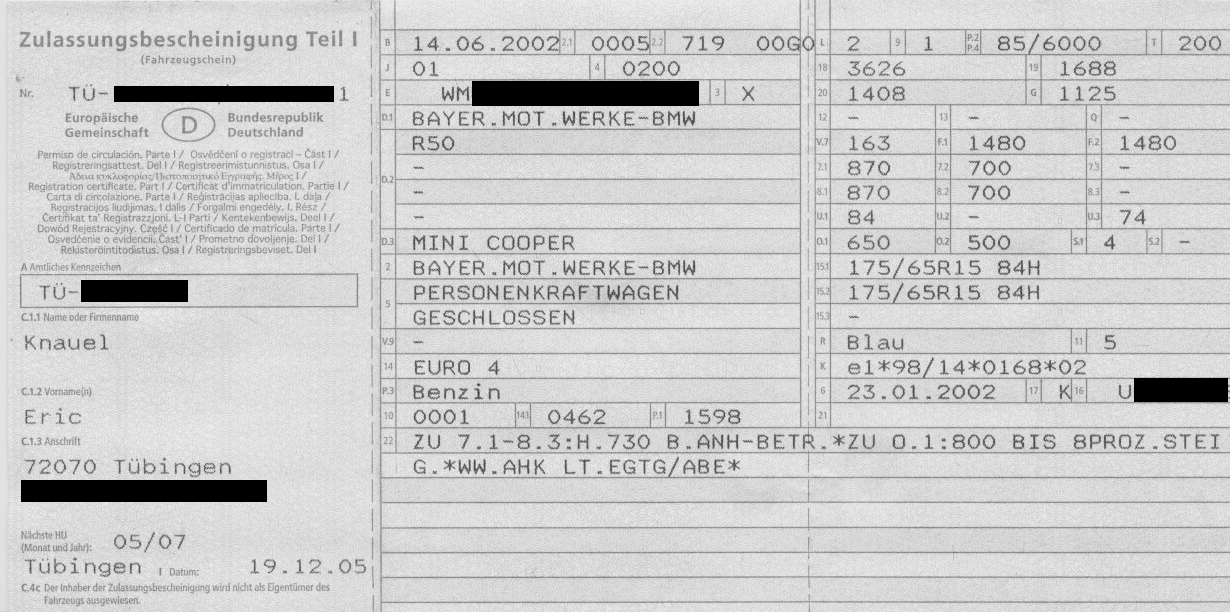
\includegraphics[width=\linewidth]{i1zus/kfzschein-front}\\
        \medskip
        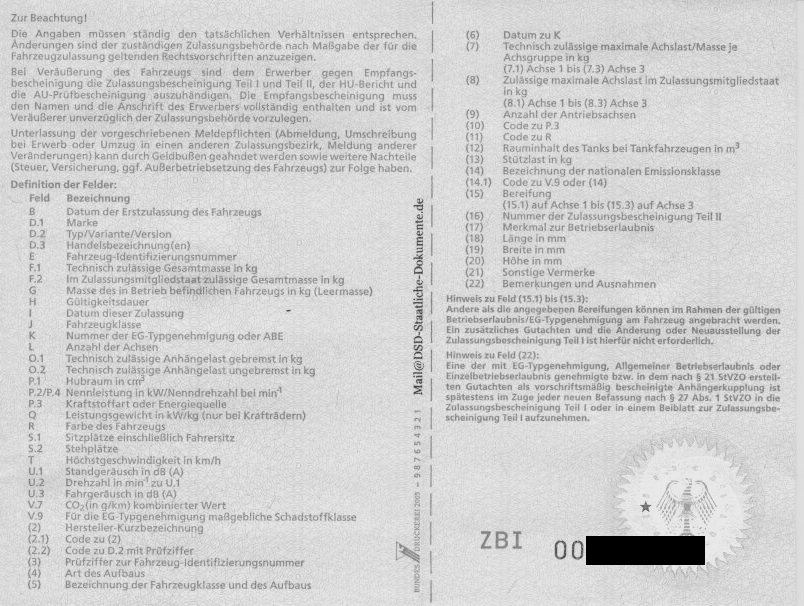
\includegraphics[width=\linewidth]{i1zus/kfzschein-back}
      \end{center}
      \caption{Vorder- und Rückseite eines Fahrzeugscheins}
      \label{fig:fahrzeugschein}
    \end{figure}
\end{aufgabe}

\begin{aufgabe}

  Schreiben Sie für den Tübinger Stadtverkehr ein
  Programm, welches überprüft ob ein Fahrzeug in den Umweltzonen fahren 
  darf.
  \begin{enumerate}
  \item Definieren Sie einen Datentyp für Fahrzeuge. Dieser
    Datentyp soll den Typ, das Nummernschild und die Schadstoffklasse des
    Fahrzeuges beinhalten.
  \item Erstellen Sie die Beispielfahrzeuge für die
    Fahrzeugtypen "'Stadtbus"', "'Reisebus"', "'Dieselauto"'
    und "'Benzinauto"'. Gehen Sie davon aus, dass die Busse der
    Schadstoffklasse~2, das Dieselauto der Schadstoffklasse~3 und das
    Benzinauto der Schadstoffklasse~4 angehören.
  \item Schreiben Sie eine Funktion \texttt{fahrverbot?},
    welche überprüft ob ein gegebenes Fahrzeug bei einer gegebenen
    Mindest-Schadstoffklasse noch fahren darf. Gestalten Sie die Signatur
    so, dass er nur Mindest-Schadstoffklassen von 1 bis 4 akzeptiert.
  \item Die Mühlstraße in Tübingen ist in einer Richtung für
    alle Fahrzeuge außer Stadtbusse gesperrt. Schreiben Sie eine Funktion
    \texttt{sonderrecht?}, die überprüft ob ein gegebenes Fahrzeug die
    Mühlstraße in der gesperrten Richtung befahren darf.  
  \item Bürgermeister Boris Palmer hat die Idee, den Tourismus
    dadurch anzukurbeln, dass Sonntags auch Reisebusse die Mühlstrasse in
    der gesperrten Richtunge befahren dürfen. Erweitern Sie hierfür die
    Funktion \texttt{sonderrecht?} um den Wochentag und lassen Sie Sonntags
    auch Reisebusse zu.
  \end{enumerate}
  Verwenden Sie beim Schreiben der Funktion die
  Konstruktionsanleitungen für Funktionen und für Fallunterscheidungen. 
  Schreiben Sie Testfälle, die alle Möglichkeiten der   
  Fallunterscheidung abdecken.
  
\end{aufgabe}

\begin{aufgabe}

  Schreiben Sie ein Programm für einen Paketdienst, das den Preis
  für ein Paket berechnet!
  \begin{enumerate}
    
  \item Schreiben Sie eine Daten- und eine Record-Definition für
    \textit{Adressen}.  Zu einer Adresse gehören der Name, die Straße
    mit Hausnummer, die Postleitzahl, der Ort und das Land.
    
  \item Der Paketdienst verlangt einen Zuschlag für Sendungen, die
    international verschickt werden.  Schreiben Sie eine Funktion
    \texttt{international?}, die als Argument eine \textit{Adresse}
    bekommt und feststellt, ob die Adresse im Ausland liegt.

  \item Der Paketdienst hat einen Sondertarif für Sendungen, die
    innerhalb der gleichen Postleitzahl verschickt werden.  Schreiben
    Sie eine Funktion \texttt{same-zip-code?}, die als Argumente zwei
    \textit{Adressen} bekommt und feststellt, ob die Postleitzahlen
    und die Länder der beiden Adressen gleich sind.

  \item Ein Paket wird klassifiziert nach seinen Abmessungen.
    Schreiben Sie eine Daten- und eine Record-Definition für
    \textit{Abmessungen}.  Abmessungen bestehen aus Länge, Breite und
    Höhe.

  \item Die Paketpreise richten sich nach der Größe des zu
    verschickenden Pakets.  Der Paketdienst verwendet die drei
    Größenklassen \textit{Small}, \textit{Medium} und \textit{Large},
    um die Kosten für das Paket zu berechnen.  Ausschlaggebendes
    Kriterium für die Paketgröße ist die Summe der längsten und der
    kürzesten Seite des Pakets.  Schreiben Sie eine Funktion
    \texttt{add-longest-and-shortest-side}, die als Argument eine
    \textit{Abmessung} bekommt.  Der Rückgabewert von
    \texttt{add"=longest"=and"=shortest"=side} soll die Summe der längsten
    und der kürzesten Seite der Abmessung sein.  Lagern Sie die
    Teilprobleme in zwei Hilfsprozeduren aus: \texttt{longest-side}
    und \texttt{shortest-side}.

  \item Schreiben Sie eine Daten- und eine Record-Definition für
    \textit{Pakete}.  Ein Paket besteht aus einer Absender- und einer
    Empfängeradresse.  Benutzen Sie für die Adressen Ihre bereits
    erstellte Record-Definition.  Außerdem hat ein Paket noch weitere
    Eigenschaften: Die Abmessungen (benutzen Sie dafür Ihre bereits
    erstellte Record-Definition), das Gewicht, die Beförderungsdauer
    und eine Zusatz\-option Nachnahme.  Die Beförderungsdauer soll
    \emph{normal}, \emph{next-day} oder \emph{next-morning} sein.

  \item Schreiben Sie eine Funktion \texttt{parcel-size-class}, die
    als Argument ein \textit{Paket} bekommt und die Größenklasse
    zurückgibt.  Ausschlaggebend für die Paketgröße ist die Abmessung
    (siehe oben).  Folgende Tabelle enthält die Zuordnung von
    Paketgröße und Abmessung:

    \begin{center}
      \begin{tabular}{c|l}
        Paketgröße & Abmessung \\
        \hline
        S & 0--50 cm \\
        M & $>$50--100 cm \\
        L & $>$100 cm \\
      \end{tabular}
    \end{center}

  \item Schreiben Sie eine Funktion \texttt{calculate-base-postage},
    die als Argument ein \textit{Paket} bekommt und die
    Basis-Portokosten für dieses Paket berechnet.  Legen Sie dabei
    folgende Grundtariftabelle des Paketdienstes zugrunde:

    \begin{center}
      \begin{tabular}{c|ccc}
        & \multicolumn{3}{c}{Gewicht} \\
        Paketgröße & 0--5 kg & $>$5--10 kg & $>$10 kg \\
        \hline
        S & 3,00 & 6,00 & 9,00 \\
        M & 6,00 & 10,00 & 14,00 \\
        L & 9,00 & 15,00 & 21,00 \\
      \end{tabular}
    \end{center}

    

  \item Schreiben Sie eine Funktion
    \texttt{transportation-time-factor}, die als Argument ein
    \textit{Paket} bekommt und den Aufschlagsfaktor für die
    Beförderungsdauer zurückliefert.  Legen Sie dabei folgende
    Aufschlagsfaktoren zugrunde:
    
    \begin{center}
      \begin{tabular}{c|ccc}
        & \multicolumn{3}{c}{Beförderungsdauer} \\
        Beförderungsdistanz & normal & next-day & next-morning \\
        \hline
        gleiche PLZ & -25\% & +0\% & +25\% \\
        Inland & +0\% & +50\% & +100\% \\
        Ausland & +100\% & +200\% & +300\% \\
      \end{tabular}
    \end{center}
    
  \item Schreiben Sie eine Funktion
    \texttt{cash-on-delivery-surcharge}, die als Argument ein
    \textit{Paket} bekommt und den Aufschlag für die Nachnahme
    zurückliefert.  Legen Sie dabei folgende Aufschläge zugrunde:

    \begin{center}
      \begin{tabular}{c|c}
        Beförderungsdistanz & Nachnahmegebühr \\
        \hline
        Inland & +3,00 \\
        Ausland & +9,00 \\
      \end{tabular}
    \end{center}

  \item Schreiben Sie eine Funktion \texttt{calculate-postage}, die
    als Argument ein \textit{Paket} bekommt und die Portokosten
    berechnet.  Benutzen Sie dafür die von Ihnen programmierten
    Lösungen der verschiedenen Teilprobleme.
    
  \end{enumerate}
  
\end{aufgabe}

\begin{aufgabe}
  \label{aufgabe:knaubichler}
  Auf seinen Reisen um die Welt trifft Dr.~Sperber
  viele interessante und skurrile Zeitgenossen. Unter ihnen
  Dr.~Knaubichler, ein Experte auf dem Gebiet der Kreuzung von
  mystischen Kreaturen.  Es gibt drei klassische Grundkreaturen:

  \begin{itemize}
  \item Der Garnolaf, der Stärke besitzt.
  \item Das Ronugor, das Wissen besitzt.
  \item Der Tschipotol, der Risikobereitschaft besitzt.
  \end{itemize}
  
  Die Merkmale der Kreaturen sind unterschiedlich ausgeprägt.  Die
  Knaubichler-Kreaturenmerkmal-Skala geht von 0 bis 100.  Die
  Grundkreaturen haben jeweils nur ein Merkmal, keine besitzt ein
  Merkmal einer anderen Grundkreatur.

  Nun kreuzt Dr.~Knaubichler die Grundkreaturen miteinander. Es
  entstehen also
  \begin{itemize}
  \item Das Ronulaf, mit Wissen und Stärke.
  \item Der Tschigor, mit Wissen und Risikobereitschaft.
  \item Das Lapotol, mit Stärke und Risikobereitschaft.
  \item Der Tschirgaronu, Wissen, Stärke und Risikobereitschaft.
  \end{itemize}
  
  Leider erben die Kreuzungen nicht die vollen Merkmale beider
  Grundkreaturen.

  Bei der Kreuzung unterschiedlicher Grunkreaturen gilt folgendes:
  Bei der Kreuzung von Ronugor und Tschipotol wird
  das übernommene Wissen um 10\% veringert; bei Tschipotol und
  Garnolaf hingegen nimmt die Risikobereitschaft um 5\% ab, aber die
  Stärke legt um 8\% zu. Garnolaf und Ronugor lassen die Stärke um 5\%
  zulegen. Kreuzt man alle drei Grundkreaturen, nimmt jede Eigenschaft
  um 3\% ab.
  
  Werden zwei Kreaturen der gleichen Sorte gekreuzt, so entsteht eine
  neue Kreatur mit $\frac{2}{3}$ der addierten Eigenschaften der
  beiden Grundkreaturen. Man kann nur Grundkreaturen kreuzen.

  In jedem Fall kann eine Eigenschaft maximal den Wert 100
  haben.
    
  Dr.~Knaubichler braucht ein Programm, welches die neue Kreatur
  berechnet, bevor er die Kreuzungen durchführt.  Helfen Sie ihm
  dabei!
  
  \begin{enumerate}

  \item Machen Sie eine Datenanalyse und erstellen
    Sie passende Daten- und Recorddefinitionen.  Geben Sie alle
    Signaturen der Record-Funktionen an!

  \item Schreiben Sie für jede der oben aufgelisteten
    Kreuzungen von zwei Grundkreaturen eine Funktion, die die Kreuzung
    vornimmt und eine neue Kreatur zurückgibt.
  \end{enumerate}
\end{aufgabe}


%%% Local Variables: 
%%% mode: latex
%%% TeX-master: "i1"
%%% End: 
